\documentclass[11pt]{article}
\usepackage{graphicx}
\usepackage{amsmath}
\usepackage{booktabs}
\usepackage{caption}
\usepackage{subcaption}
\usepackage{hyperref}
\usepackage{float}
\usepackage{geometry}
\geometry{margin=1in}
\usepackage{algorithm}
\usepackage{algpseudocode}

\title{SC4003 Assignment 1: Agent Decision Making}
\author{Aloysius Tan U2120998C}
\date{\today}

\begin{document}

\makeatletter
\begin{titlepage}
\begin{center}


\includegraphics[width=\textwidth]{ntu_logo.png} 
\\[1cm]

\uppercase{\textbf{\large{Nanyang Technological University}}}
\\[6cm]

\uppercase{\textbf{\large{\@title}}}

\vfill
\@author
\\[3cm]

College of Computing and Data Science

\@date

\end{center}
\end{titlepage}
\makeatother


% \addcontentsline{toc}{chapter}{Contents}
\tableofcontents
\newpage 

\section{Introduction}
This report presents the implementation and analysis of Markov Decision Processes (MDPs) for
solving maze environments. Two algorithms are implemented and compared: Value Iteration
and Policy Iteration, as described in Chapter 17 of \emph{Artificial Intelligence: A Modern Approach (3rd ed.)}~\cite{AIMA}, which introduces Markov Decision Processes, Bellman updates, and iterative solution algorithms.


\noindent We conduct experiments on maze environments of different sizes and complexities, ranging from a small 6x6 layout to a large 20x20 grid. Each maze cell can be:
\begin{itemize}
    \item \textbf{Empty} (white cell with a small negative reward, e.g., $-0.05$),
    \item \textbf{Goal} (green cell with a positive reward, e.g., $+1$),
    \item \textbf{Penalty} (orange cell with a negative reward, e.g., $-1$),
    \item \textbf{Wall} (black cell that are impassable),
    \item \textbf{Start} (blue cell where the agent begins).
\end{itemize}
The key questions are how the number of states and the maze's structural complexity (i.e., arrangement of walls and reward cells) affect the convergence rates and computational costs of VI and PI.

\section{Part 1: Standard Maze (6x6)}
\label{sec:part1}

In the reference material (Sections~2.1--2.4), a small maze is used to illustrate fundamental concepts of Value Iteration and Policy Iteration. Here, we replicate that approach with a \textbf{6x6 maze} containing:
\begin{itemize}
    \item White squares (reward $-0.05$),
    \item One or more goal squares ($+1$),
    \item Penalty squares ($-1$),
    \item Walls (impassable),
    \item A designated start cell (also $-0.05$).
\end{itemize}

\subsection{6x6 Maze Layout}
Figure~\ref{fig:maze6x6} shows the 6x6 environment. This layout is fixed (hard-coded), analogous to the standard example from the PDF.

\begin{figure}[H]
    \centering
    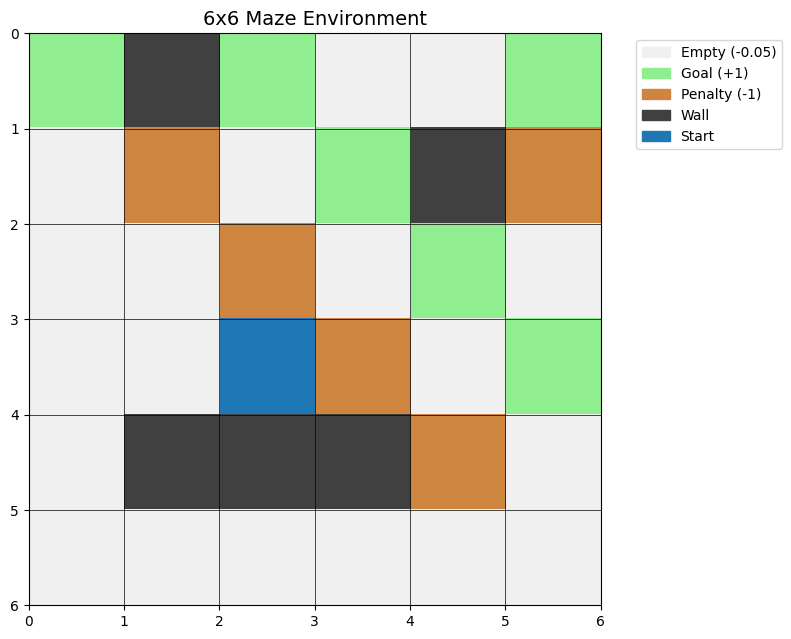
\includegraphics[width=0.85\textwidth]{maze_6x6_environment.png}
    \caption{6x6 Maze Environment}
    \label{fig:maze6x6}
\end{figure}

\subsection{Value Iteration}
\label{sec:vi_6x6}
Value Iteration is a Reinforcement Learning algorithm to eventually find the optimal policy for a system modeled as a Markov Decision Process (MDP) by iteratively making adjustments to the utility function. This function measures how desirable the current state is. The central idea is to use the Bellman update rule to update the utility values of each state until we converge to an optimal value.
\[
U(s) \leftarrow R(s) + \gamma \max_a \sum_{s'} P(s' \mid s,a)\,U(s').
\]
This process continues until the maximum change in utility values across states falls below a small threshold (e.g., $10^{-6}$) or a maximum iteration limit is reached. 

\begin{algorithm}
\caption{Value Iteration}
\label{alg:value_iteration}
\begin{algorithmic}[1]
    \Function{Value\_Iteration}{$mdp, \epsilon, max\_iterations$}
        \State \textbf{inputs:} $mdp$, an MDP with states $S$, actions $A(s)$, transition model $P(s'|s,a)$
        \State \hspace{11mm} rewards $R(s)$, discount factor $\gamma$, threshold $\epsilon$, max iteration limit
        \State \textbf{local variables:} 
        \Indent
            \State $U$, $U'$, vectors of utilities for states in $S$, initially zero
            \State $\delta$, the maximum change in utility of any state in an iteration
            \State $iterations \gets 0$
        \EndIndent
        \Repeat
            \State $U \gets U'$
            \State $\delta \gets 0$
            \For {each state $s \in S$}
                \State Compute expected utility for all actions:
                \[
                Q(s, a) = \sum_{s'} P(s' | s, a) U(s')
                \]
                \State $U'[s] \gets R(s) + \gamma \max\limits_{a} Q(s, a)$
                \State $\delta \gets \max(\delta, |U'[s] - U[s]|)$
            \EndFor
            \State $iterations \gets iterations + 1$
        \Until {$\delta < \epsilon$ or $iterations \geq max\_iterations$}
        \State \Return $U$
    \EndFunction
\end{algorithmic}
\end{algorithm}

\newpage
\subsubsection{Descriptions of Implemented Solutions}
We implement Value Iteration (\textbf{VI}) for the 6x6 maze as follows:
\begin{enumerate}
    \item \textbf{Initialization:} Set the utility $U(s) = 0$ for all states $s$ and initialize an empty policy.
    \item \textbf{Iterative Updates:} For each state $s$, update its utility using the Bellman optimality equation:
    \[
    U(s) \leftarrow R(s) + \gamma \max_a \sum_{s'} P(s' \mid s,a)\,U(s'),
    \]
    where $R(s)$ is the immediate reward for state $s$, $\gamma$ is the discount factor, and $P(s' \mid s,a)$ represents the transition probabilities.
    \item \textbf{Convergence Check:} After each full update over the state space, compute the maximum change in utility. If this change is less than $10^{-6}$, or if a preset iteration limit is reached, the algorithm terminates.
    \item \textbf{Recording Trajectories:} The utility values for all states are recorded at each iteration, allowing us to generate convergence plots showing how the utilities evolve over time.
\end{enumerate}

\newpage
\noindent The implementation of Value Iteration is provided in the file \texttt{mdp\_solution.py}. The function \texttt{value\_iteration} is responsible for iteratively applying the Bellman backup and updating utilities until convergence. The complete implementation is provided below:

\begin{verbatim}
def value_iteration(self, max_iterations=1000, threshold=1e-6, return_metrics=False):
    """
    Value iteration to find optimal utilities & policy.
    Optionally returns performance metrics: iterations, total time, 
    and Bellman backup count.
    """
    utilities = {s: 0.0 for s in self.states}
    policy = {s: 0 for s in self.states}
    utility_history = [utilities.copy()]
    bellman_backups = 0
    start_time = time.time()
    iteration = 0

    while iteration < max_iterations:
        max_change = 0
        new_utilities = utilities.copy()
        for state in self.states:
            bellman_backups += 1  # Count each state update as one backup.
            i, j = state
            action_values = []
            for a in self.actions:
                transitions = self.get_transition_probs(state, a)
                exp_util = sum(prob * utilities[s_next] for s_next, prob in transitions)
                action_values.append(self.rewards[i, j] + self.discount_factor * exp_util)
            best_action_value = max(action_values)
            best_action = np.argmax(action_values)
            new_utilities[state] = best_action_value
            policy[state] = best_action
            max_change = max(max_change, abs(best_action_value - utilities[state]))
        utilities = new_utilities
        utility_history.append(utilities.copy())
        
        if max_change < threshold:
            break
        iteration += 1

    total_time = time.time() - start_time
    print(f"Value iteration converged after {iteration} iterations (threshold={threshold})")
    if return_metrics:
        metrics = {"iterations": iteration, "time": total_time, 
            "bellman_backups": bellman_backups}
        return utilities, policy, utility_history, metrics
    else:
        return utilities, policy, utility_history
\end{verbatim}

\subsubsection{Plot of Optimal Policy and Utilities of All States}
Figure~\ref{fig:6x6_vi_side_by_side} displays the final Value Iteration policy (with overlaid arrows) and the corresponding utility map using the environment's color scheme. 

\begin{figure}[H]
    \centering
    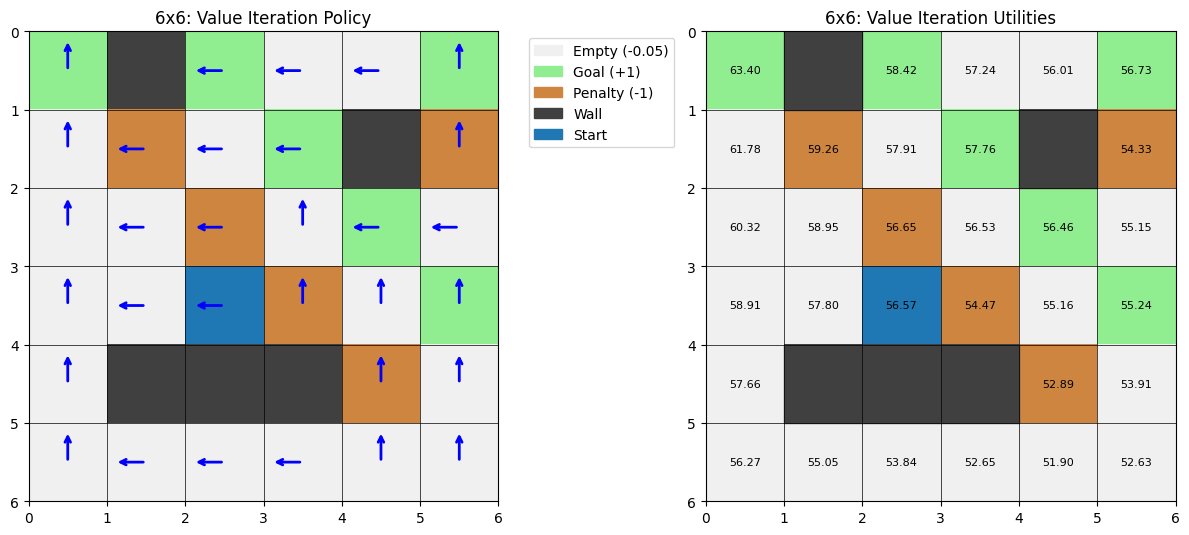
\includegraphics[width=0.75\textwidth]{6x6_value_iteration.png}
    \caption{Final Value Iteration Policy (left) and Value Utilities (right) for the 6x6 Maze. The image displays the environment color scheme with overlaid arrows and utility values.}
    \label{fig:6x6_vi_side_by_side}
\end{figure}

\subsubsection{Plot of Utility Estimates vs. Iterations}
Figure~\ref{fig:6x6_vi_convergence} shows the convergence trajectories of the utilities across iterations.
\begin{figure}[H]
    \centering
    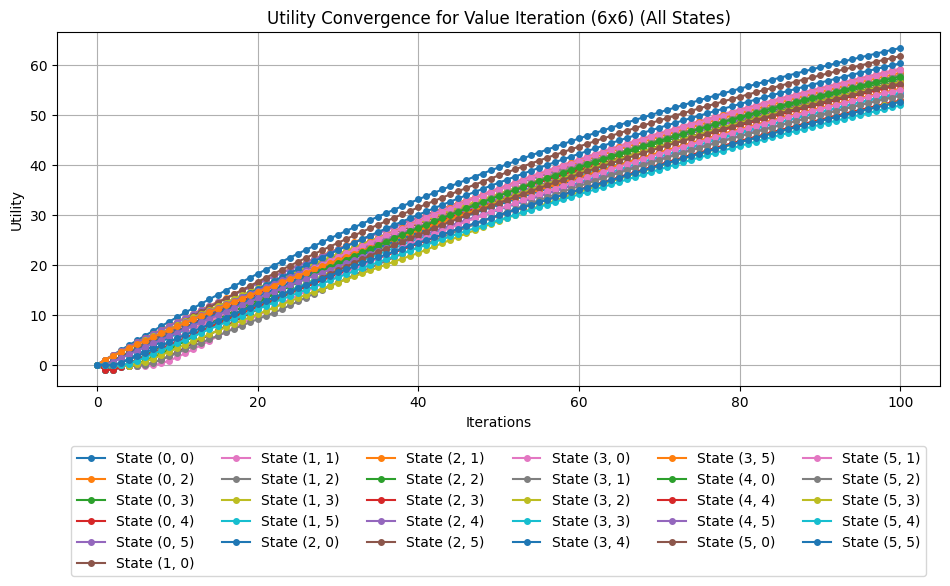
\includegraphics[width=0.75\textwidth]{6x6_value_iteration_convergence.png}
    \caption{Utility Convergence for Value Iteration (6x6). Each colored line represents one state's utility across iterations.}
    \label{fig:6x6_vi_convergence}
\end{figure}

\newpage
\subsection{Policy Iteration: Implementation and Results}
\label{sec:pi_6x6}
Policy Iteration is a classical algorithm used to solve Markov Decision Processes (MDPs). It works by alternating between two main steps: policy evaluation and policy improvement. Given an initial random policy, the algorithm evaluates the utility of each state under the current policy, then improves the policy by choosing actions that maximize the expected utility. This process repeats until convergence.

\begin{algorithm}
\caption{Policy Iteration}
\label{alg:policy_iteration}
\begin{algorithmic}[1]
\Function{Policy-Iteration}{$mdp$}
    \State \textbf{inputs:} $mdp$, an MDP with states $S$, actions $A(s)$, transition model $P(s'|s,a)$, reward function $R(s)$, discount factor $\gamma$
    \State \textbf{local variables:} 
    \Indent
        \State $U$, a vector of utilities for states in $S$, initially set to $0$
        \State $\pi$, a policy vector indexed by state, initially assigned random actions across all valid states
    \EndIndent
    \Repeat
        % \tcp{Policy Evaluation}
        \State $U \gets$ \Call{Policy-Evaluation}{$\pi, U, mdp$}
        \State $policy\_stable \gets$ \textbf{True}
        
        % \tcp{Policy Improvement}
        \For{each state $s$ in $S$}
            \State $old\_action \gets \pi[s]$
            \State $\pi[s] \gets \arg\max_{a \in A(s)} \left[ R(s) + \gamma \sum_{s'} P(s'|s,a) U[s'] \right]$
            \If{$old\_action \neq \pi[s]$}
                \State $policy\_stable \gets$ \textbf{False}
            \EndIf
        \EndFor
    \Until{$policy\_stable$ or maximum iterations reached}
    \State \textbf{return} $\pi$
\EndFunction
\end{algorithmic}
\end{algorithm}

\newpage
\subsubsection{Descriptions of Implemented Solutions}
We implement Policy Iteration (\textbf{PI}) for the 6x6 maze as follows:
\begin{enumerate}
    \item \textbf{Initialization:} We begin with an arbitrary policy $\pi_0$ that assigns a random action to each valid state. The utility of each state $U(s)$ is initialized to 0.
    \item \textbf{Policy Evaluation:} For a given policy $\pi_k$, we iteratively approximate the utilities of all states using a fixed number of iterations. The Bellman expectation equation is applied at each step:
    \[
    U(s) \leftarrow R(s) + \gamma \sum_{s'} P(s' \mid s, \pi_k(s))\, U(s').
    \]
    \item \textbf{Policy Improvement:} Once utility values are computed, we update the policy by selecting the action $a$ that maximizes expected future rewards:
    \[
    R(s) + \gamma \sum_{s'} P(s' \mid s,a)\,U(s').
    \]
    The optimal action is determined by evaluating the expected return for all available actions and selecting the one with the highest value.
    \item \textbf{Iteration Count and Convergence:} We repeat the policy evaluation and improvement steps until the policy stabilizes or a predefined iteration limit is reached.
\end{enumerate}
Throughout this process, we record the utility of every state at each iteration, enabling us to plot the utility estimates over time.

\newpage
\noindent The implementation of Policy Iteration is provided in the file \texttt{mdp\_solution.py}. The relevant function, \texttt{policy\_iteration}, is responsible for executing both policy evaluation and policy improvement steps. The full implementation is provided below:

\begin{verbatim}
def policy_iteration(self, max_iterations=100, eval_iterations=20):
    """
    Policy iteration: repeatedly evaluate and improve policy until stable.
    Returns:
        utilities (dict): final utility values
        policy (dict): final policy
        utility_history (list): utilities over iterations
    """
    # Initialize a random policy
    policy = {s: np.random.choice(self.actions) for s in self.states}
    utilities = {s: 0.0 for s in self.states}
    utility_history = [utilities.copy()]

    stable = False
    iteration = 0
    while not stable and iteration < max_iterations:
        # 1) Policy evaluation
        utilities = self._policy_evaluation(policy, utilities, eval_iterations)
        utility_history.append(utilities.copy())

        # 2) Policy improvement
        stable = True
        for state in self.states:
            i, j = state
            old_action = policy[state]

            # Find best action under current utilities
            action_values = []
            for a in self.actions:
                transitions = self.get_transition_probs(state, a)
                exp_util = sum(prob * utilities[s_next] for s_next, prob in transitions)
                action_values.append(self.rewards[i, j] + self.discount_factor * exp_util)

            best_action = np.argmax(action_values)
            if best_action != old_action:
                policy[state] = best_action
                stable = False

        iteration += 1

    print(f"Policy iteration converged after {iteration} iterations")
    return utilities, policy, utility_history
\end{verbatim}

\newpage
\subsubsection{Plot of Utility Estimates vs. Iterations}
Figure~\ref{fig:6x6_pi_convergence} shows how each state's utility evolves during the policy evaluation/improvement cycles. As the policy stabilizes, the utility curves flatten, indicating convergence. Each line corresponds to a particular state's utility across iterations. Notice how states near the goal cells converge to higher utilities, while states near penalties converge to lower values.

\begin{figure}[H]
    \centering
    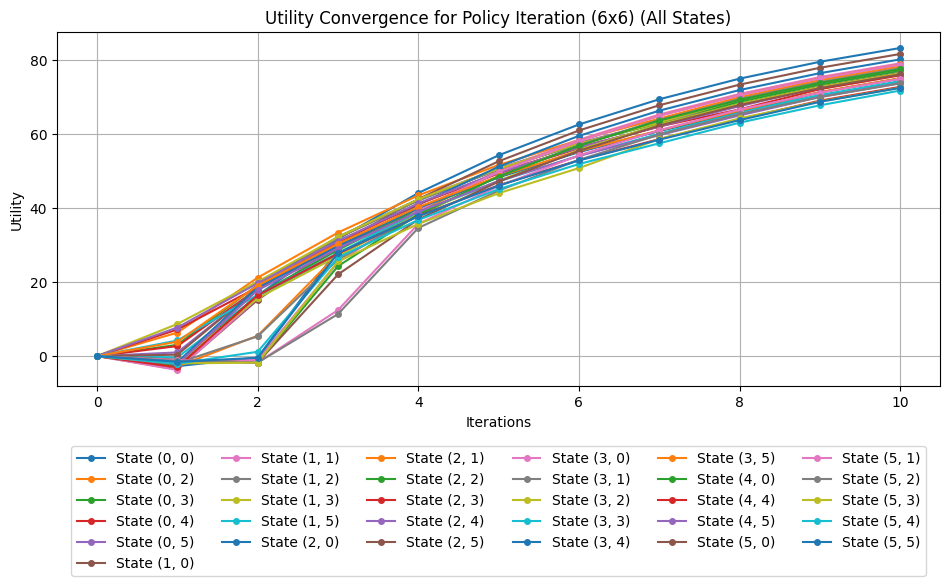
\includegraphics[width=\textwidth]{6x6_policy_iteration_convergence.png}
    \caption{Utility Convergence for Policy Iteration (6x6)}
    \label{fig:6x6_pi_convergence}
\end{figure}

\newpage
\subsubsection{Plot of Optimal Policy and Utilities of All States}
After computing the final policy $\pi^*$, we visualize it by drawing arrows in each non-wall cell indicating the optimal action. Figure~\ref{fig:6x6_pi_policy} shows the final policy for the 6x6 maze after convergence. Each arrow indicates the best action in that state. Notice how the agent is guided toward green (reward) cells and away from brown (penalty) cells.

\begin{figure}[H]
    \centering
    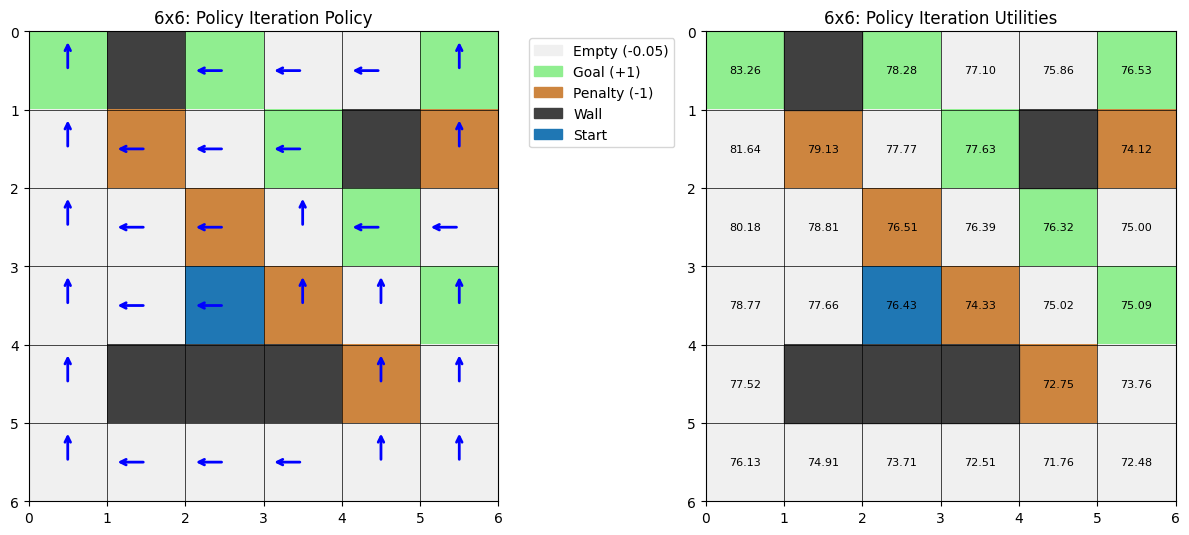
\includegraphics[width=\textwidth]{6x6_policy_iteration.png}
    \caption{Final Policy Iteration Policy for the 6x6 Maze}
    \label{fig:6x6_pi_policy}
\end{figure}

\newpage
\section{Part 2: More Complex Maze Environments}
\label{sec:part2}
We now investigate how these algorithms scale when the maze grows from 6x6 to \textbf{10x10}, \textbf{15x15}, and \textbf{20x20}. Each larger maze contains more cells, additional obstacles, and multiple goals or penalties, creating a more complex reward landscape and transition structure.

\subsection{Random Maze Generation}
While the 6x6 layout is fixed, the 10x10, 15x15, and 20x20 mazes are generated randomly using a custom function:
\begin{verbatim}
def generate_random_maze(n, m, seed=None, 
                         p_white=0.6, p_green=0.1, 
                         p_brown=0.1, p_wall=0.2):
    """
    Generate an n x m maze:
      0 = white square (-0.05)
      1 = green square (+1)
      2 = brown square (-1)
      3 = wall
      4 = start

    The outer boundary is set to walls (3).
    Each interior cell is assigned [0,1,2,3] 
    according to the given probabilities.
    One random interior cell is designated as start (4).
    """
    ...
\end{verbatim}

\noindent The parameters \verb|p_white|, \verb|p_green|, \verb|p_brown|, and \verb|p_wall| define the probability of each interior cell becoming an empty cell, goal, penalty, or wall, respectively. The function also seeds the random number generator for reproducibility and ensures the maze boundary is all walls. Finally, one random interior cell is overridden to be the start position (4).

\paragraph{Effects of Random Maze Layouts on Learning}
The randomness in maze generation introduces variations in difficulty:
\begin{itemize}
    \item \textbf{Highly structured mazes (long corridors, large open spaces)} tend to converge faster.
    \item \textbf{Dense obstacles (many walls and penalty zones)} slow down policy learning, as fewer paths exist for reward propagation.
    \item \textbf{Different random seeds lead to significant variance in convergence times} across otherwise identical maze sizes.
\end{itemize}
The randomized maze approach helps assess the robustness of VI and PI under varying environmental complexities.


\newpage
\subsection{Maze Layouts}
Figures~\ref{fig:maze10x10}--\ref{fig:maze20x20} show sample layouts for the 10x10, 15x15, and 20x20 mazes, each generated via the above randomization procedure. 

\begin{figure}[H]
    \centering
    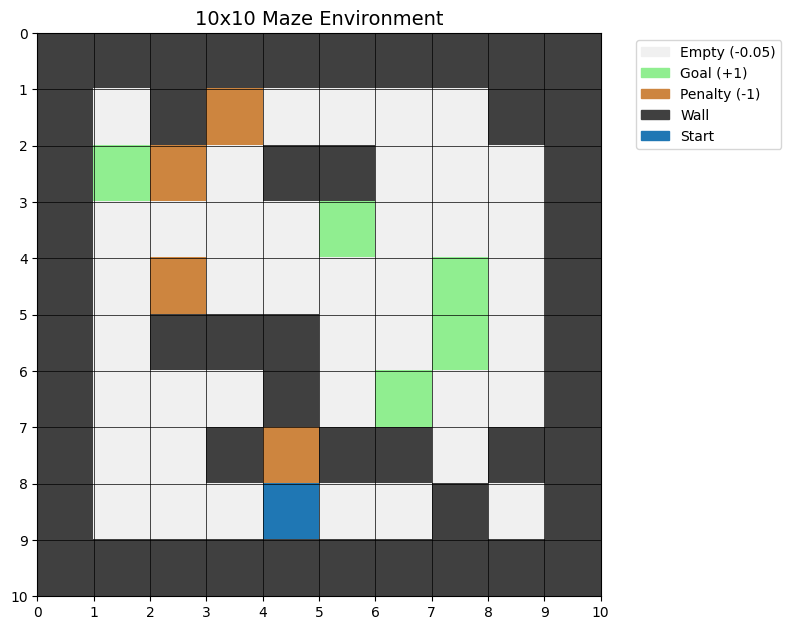
\includegraphics[width=\textwidth]{maze_10x10_environment.png}
    \caption{Randomly Generated 10x10 Maze.}
    \label{fig:maze10x10}
\end{figure}

\begin{figure}[H]
    \centering
    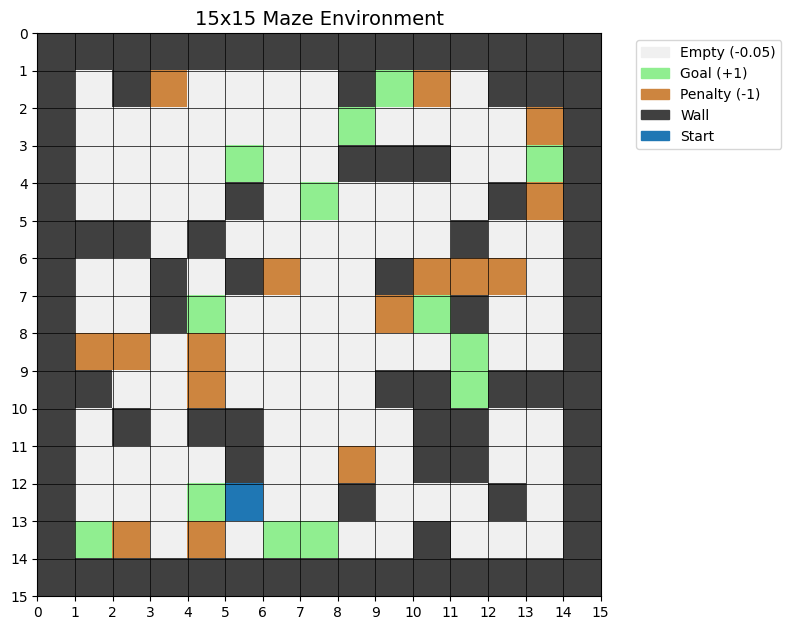
\includegraphics[width=\textwidth]{maze_15x15_environment.png}
    \caption{Randomly Generated 15x15 Maze.}
    \label{fig:maze15x15}
\end{figure}

\begin{figure}[H]
    \centering
    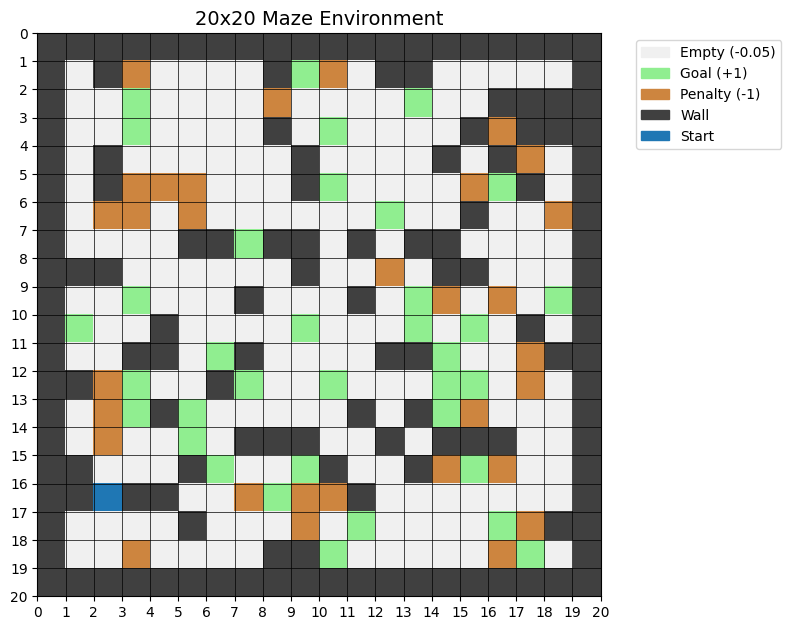
\includegraphics[width=\textwidth]{maze_20x20_environment.png}
    \caption{Randomly Generated 20x20 Maze.}
    \label{fig:maze20x20}
\end{figure}

\subsection{Convergence Trends with Increasing Size}
As the maze size and complexity grow, both VI and PI require more computational effort. The following plots illustrate how the utility estimates converge for each algorithm at 10x10, 15x15, and 20x20 scales. In each case, the final policy remains optimal, but the number of iterations (and total Bellman backups) grows substantially.

\subsubsection{10x10 Maze Results}
\begin{figure}[H]
    \centering
    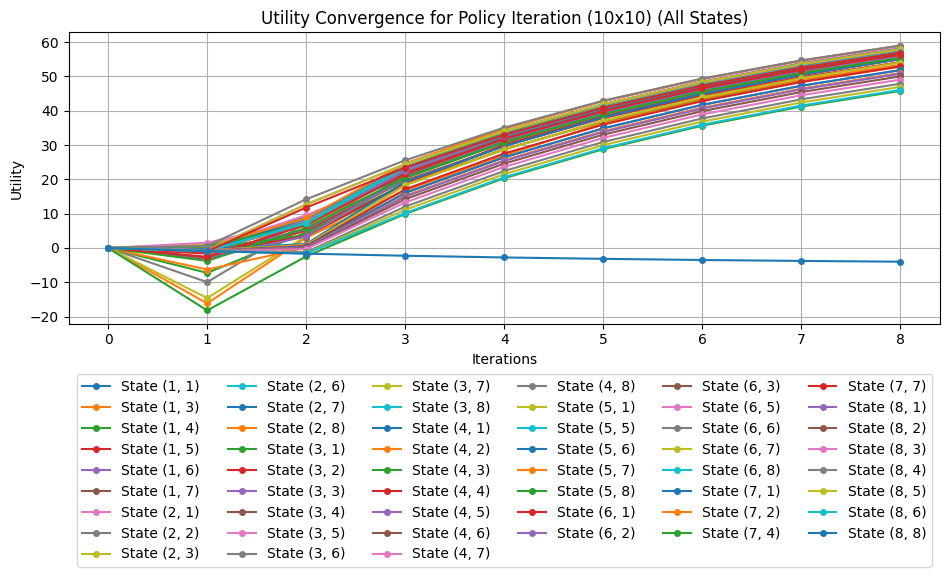
\includegraphics[width=\textwidth]{10x10_policy_iteration_convergence.png}
    \caption{Policy Iteration Convergence (10x10). Each line is a different state's utility over iterations.}
    \label{fig:10x10_pi_conv}
\end{figure}

\begin{figure}[H]
    \centering
    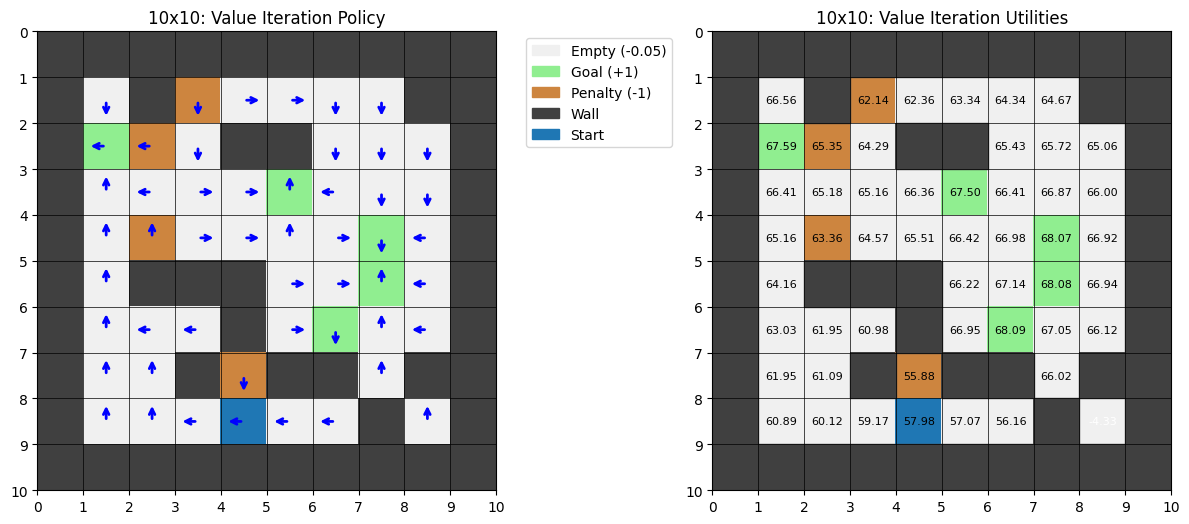
\includegraphics[width=\textwidth]{10x10_value_iteration.png}
    \caption{Final Value Iteration Policy (left) and Utilities (right) for the 10x10 Maze.}
    \label{fig:10x10_vi_side_by_side}
\end{figure}

\begin{figure}[H]
    \centering
    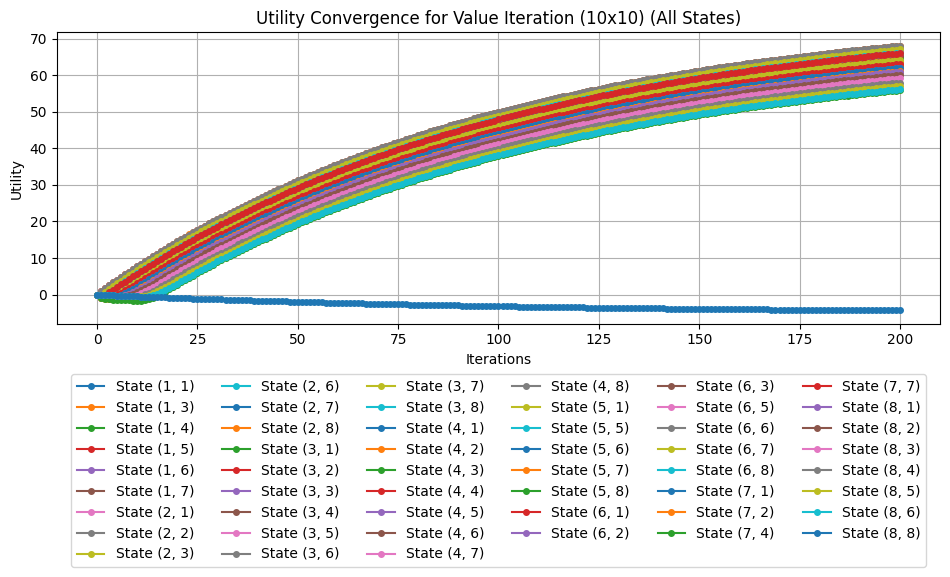
\includegraphics[width=\textwidth]{10x10_value_iteration_convergence.png}
    \caption{Value Iteration Convergence (10x10). Up to 200 iterations were used.}
    \label{fig:10x10_vi_conv}
\end{figure}

% --- New Policy Iteration final image for 10x10 ---
\begin{figure}[H]
    \centering
    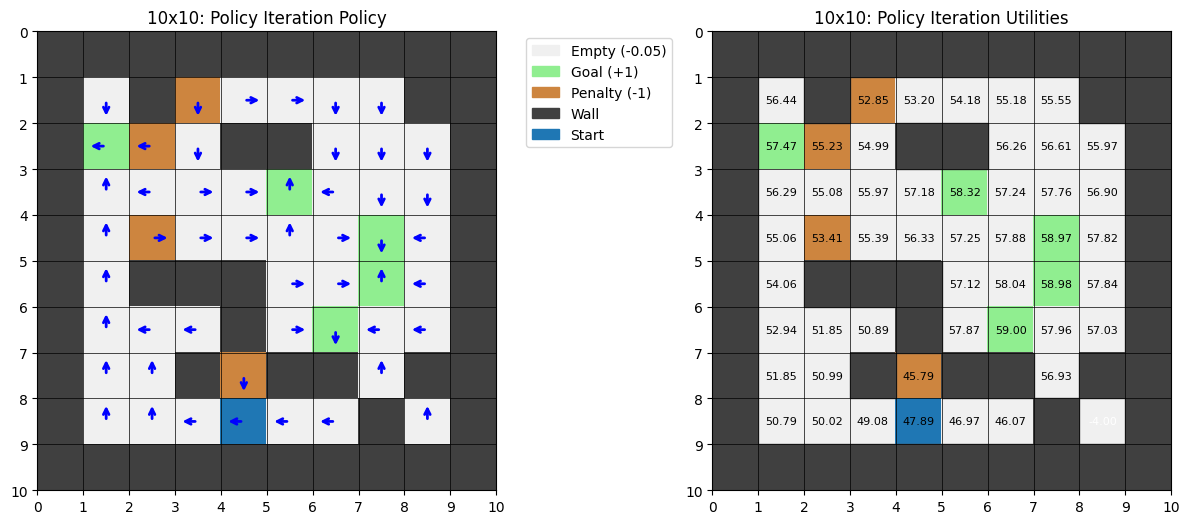
\includegraphics[width=\textwidth]{10x10_policy_iteration.png}
    \caption{Final Policy Iteration Policy and Utilities for the 10x10 Maze. This side-by-side image shows the optimal policy (arrows) and the converged utility values over the maze grid.}
    \label{fig:10x10_pi_side_by_side}
\end{figure}

\subsubsection{15x15 Maze Results}
\begin{figure}[H]
    \centering
    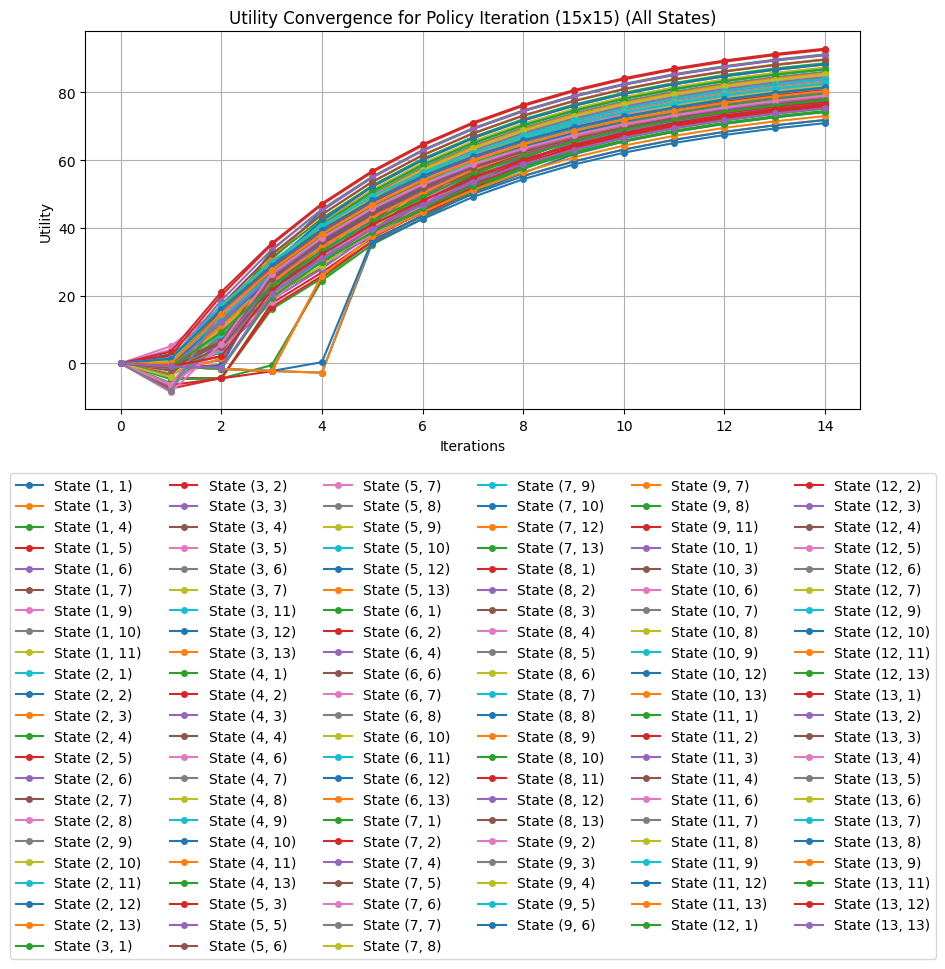
\includegraphics[width=0.65\textwidth]{15x15_policy_iteration_convergence.png}
    \caption{Policy Iteration Convergence (15x15). The increased complexity leads to more variation in utility curves.}
    \label{fig:15x15_pi_conv}
\end{figure}

\begin{figure}[H]
    \centering
    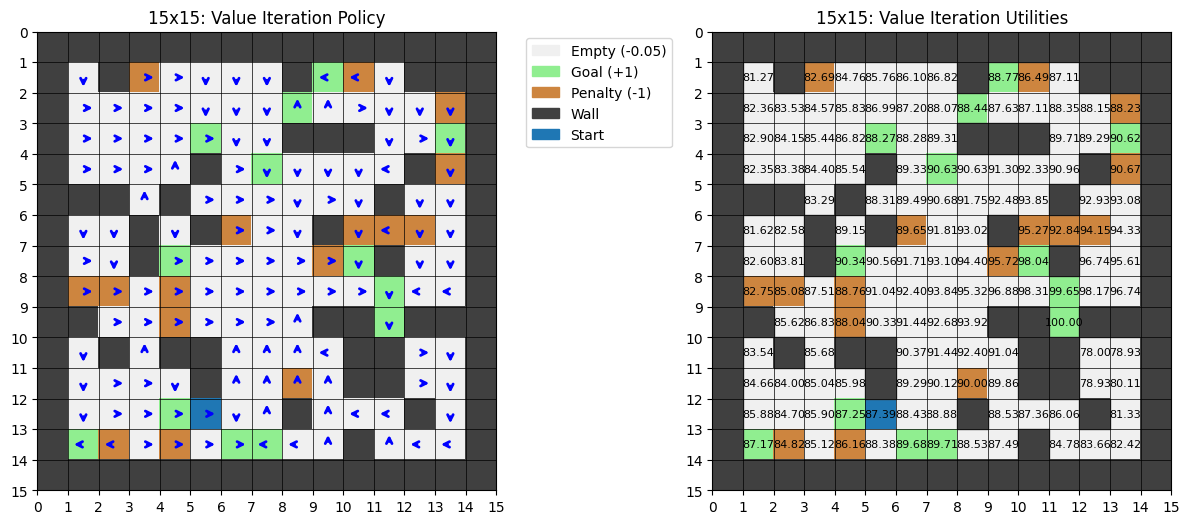
\includegraphics[width=\textwidth]{15x15_value_iteration.png}
    \caption{Final Value Iteration Policy (left) and Utilities (right) for the 15x15 Maze.}
    \label{fig:15x15_vi_side_by_side}
\end{figure}

\begin{figure}[H]
    \centering
    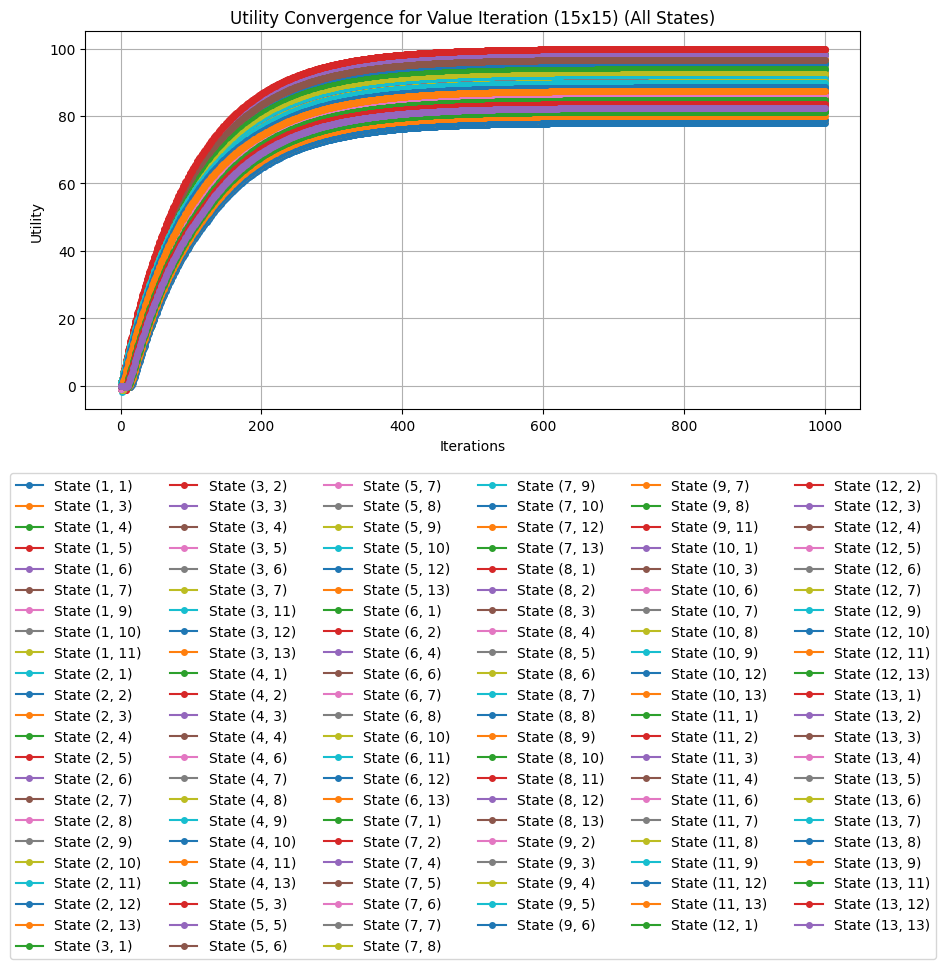
\includegraphics[width=0.65\textwidth]{15x15_value_iteration_convergence.png}
    \caption{Value Iteration Convergence (15x15). Up to 1000 iterations ensure convergence below $10^{-6}$.}
    \label{fig:15x15_vi_conv}
\end{figure}

% --- New Policy Iteration final image for 15x15 ---
\begin{figure}[H]
    \centering
    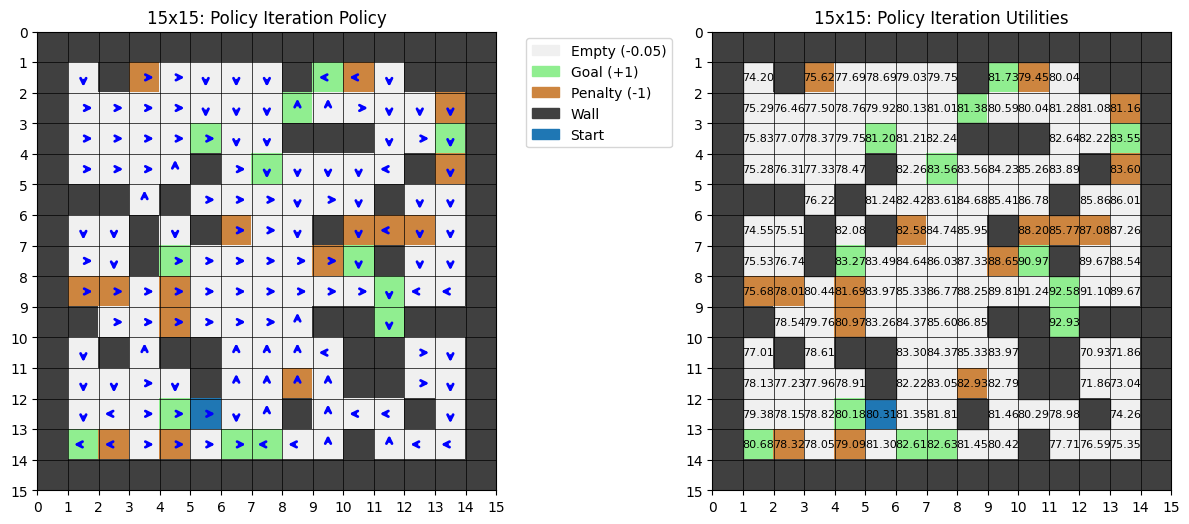
\includegraphics[width=\textwidth]{15x15_policy_iteration.png}
    \caption{Final Policy Iteration Policy and Utilities for the 15x15 Maze. The image illustrates the optimal actions (arrows) and corresponding state utilities over the maze grid.}
    \label{fig:15x15_pi_side_by_side}
\end{figure}

\subsubsection{20x20 Maze Results}
\begin{figure}[H]
    \centering
    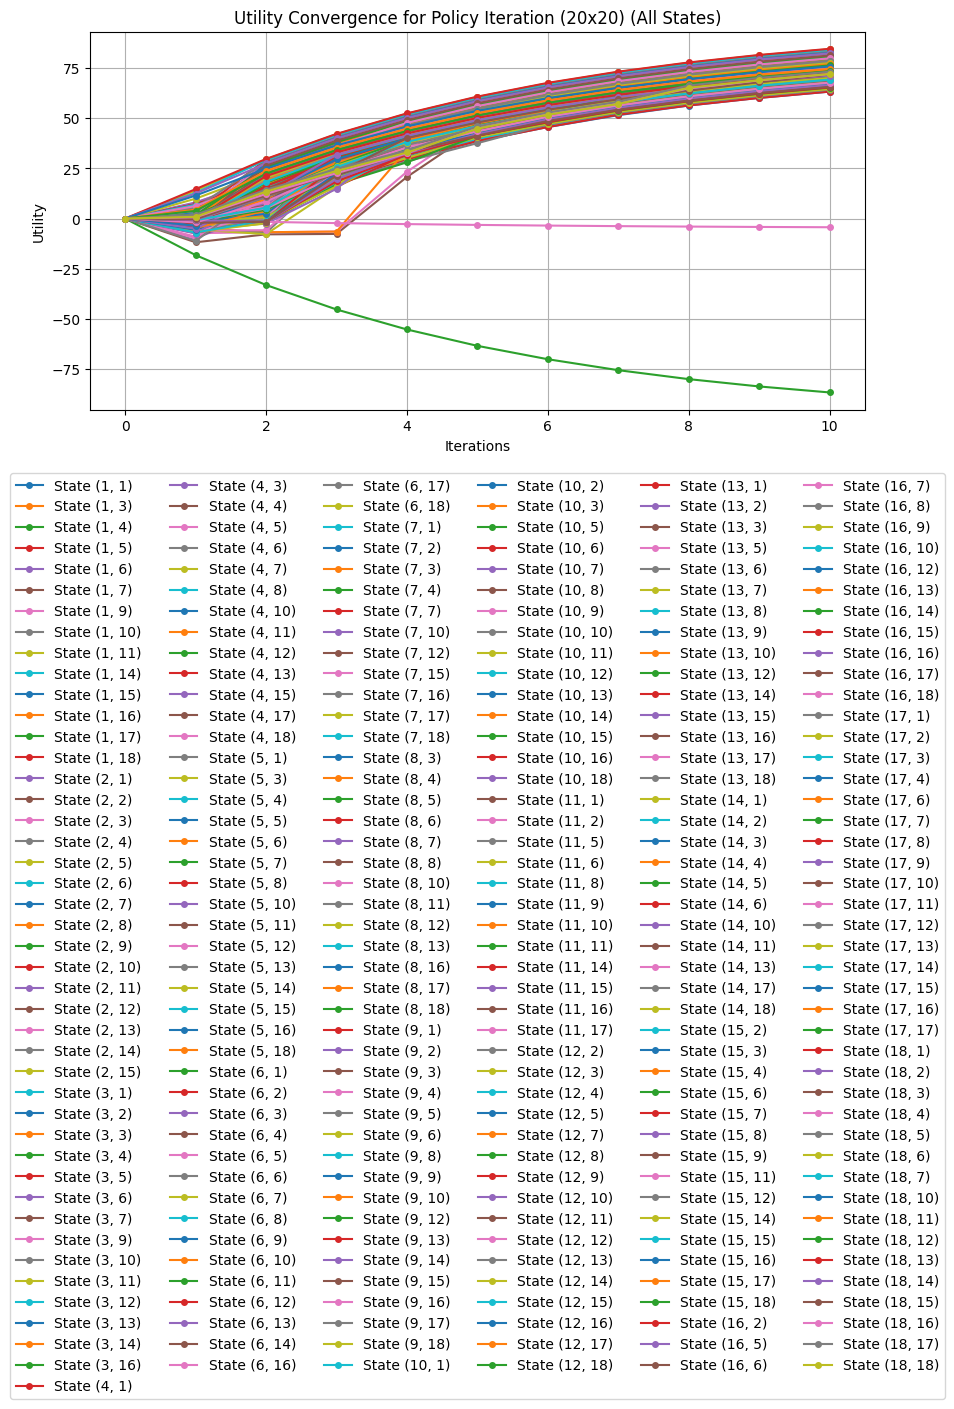
\includegraphics[width=0.8\textwidth]{20x20_policy_iteration_convergence.png}
    \caption{Policy Iteration Convergence (20x20). The large state space leads to more computationally expensive evaluation steps.}
    \label{fig:20x20_pi_conv}
\end{figure}

\begin{figure}[H]
    \centering
    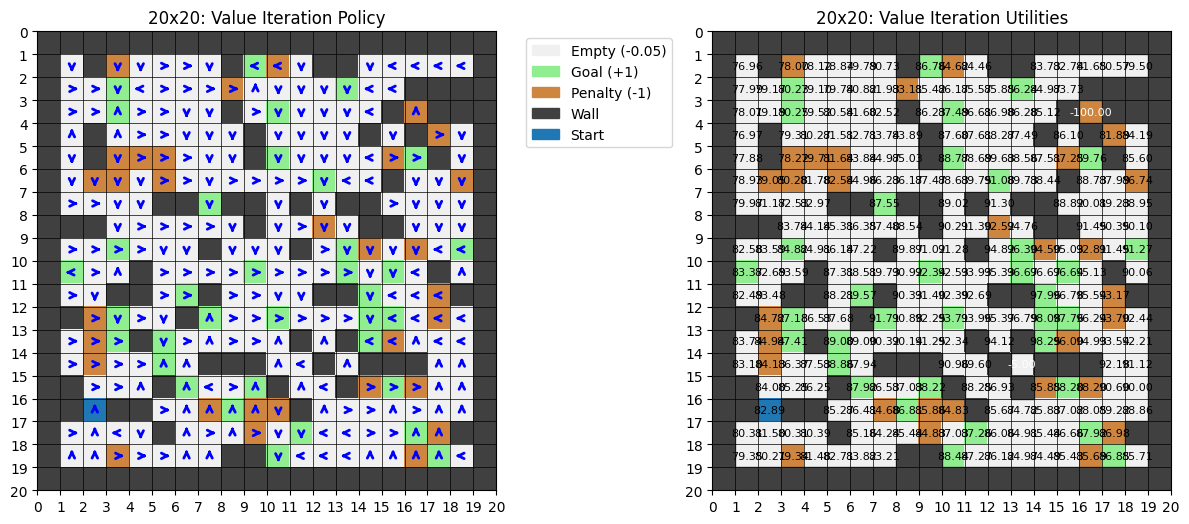
\includegraphics[width=\textwidth]{20x20_value_iteration.png}
    \caption{Final Value Iteration Policy (left) and Utilities (right) for the 20x20 Maze.}
    \label{fig:20x20_vi_side_by_side}
\end{figure}

\begin{figure}[H]
    \centering
    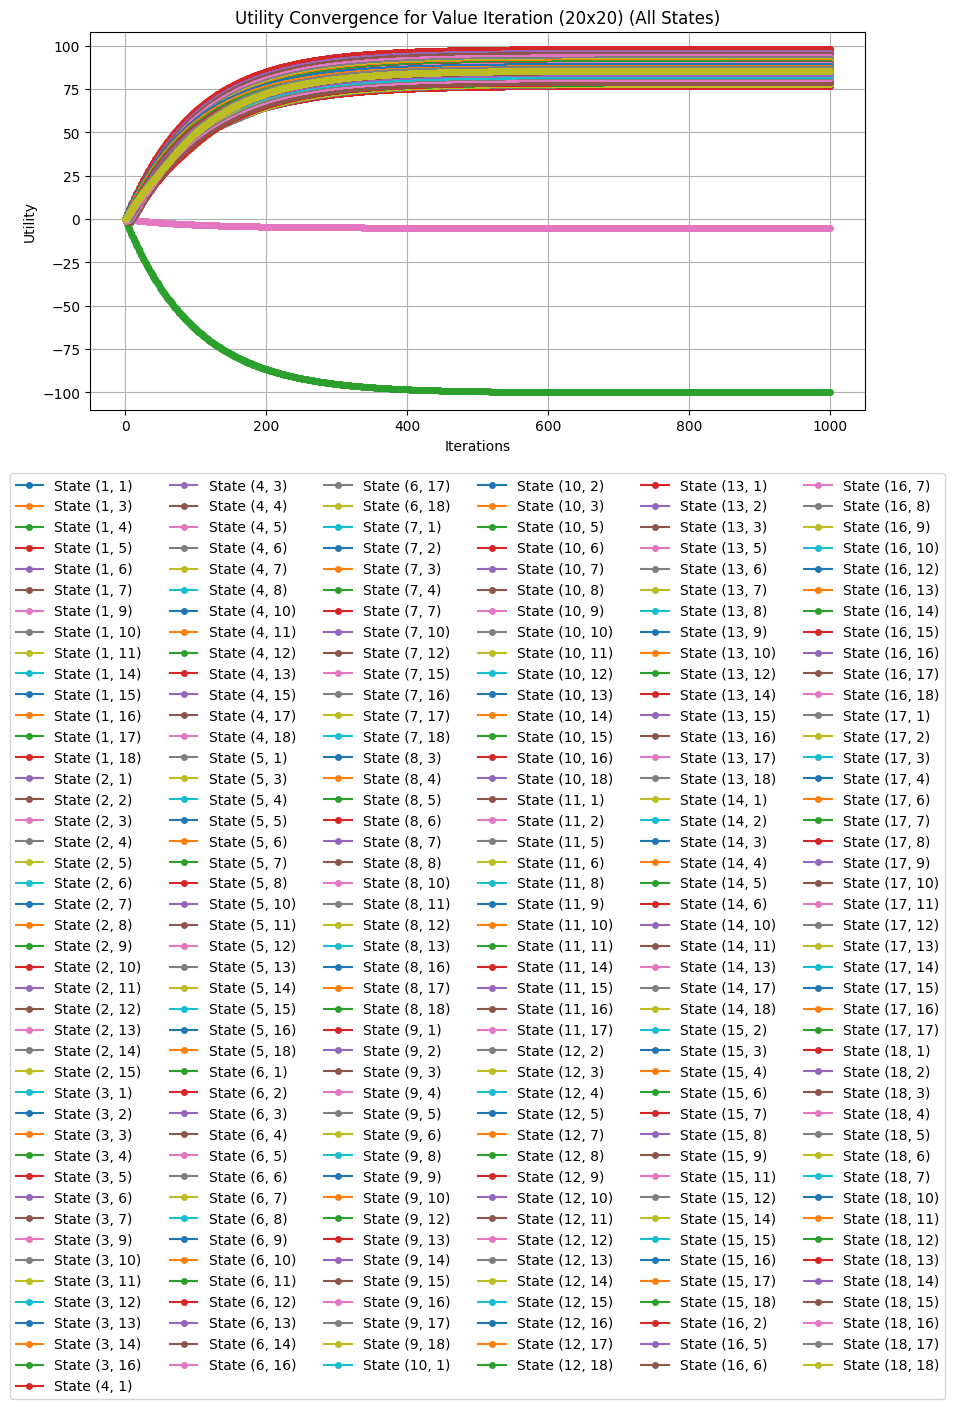
\includegraphics[width=0.8\textwidth]{20x20_value_iteration_convergence.png}
    \caption{Value Iteration Convergence (20x20). Some states require several hundred iterations to stabilize.}
    \label{fig:20x20_vi_conv}
\end{figure}

% --- New Policy Iteration final image for 20x20 ---
\begin{figure}[H]
    \centering
    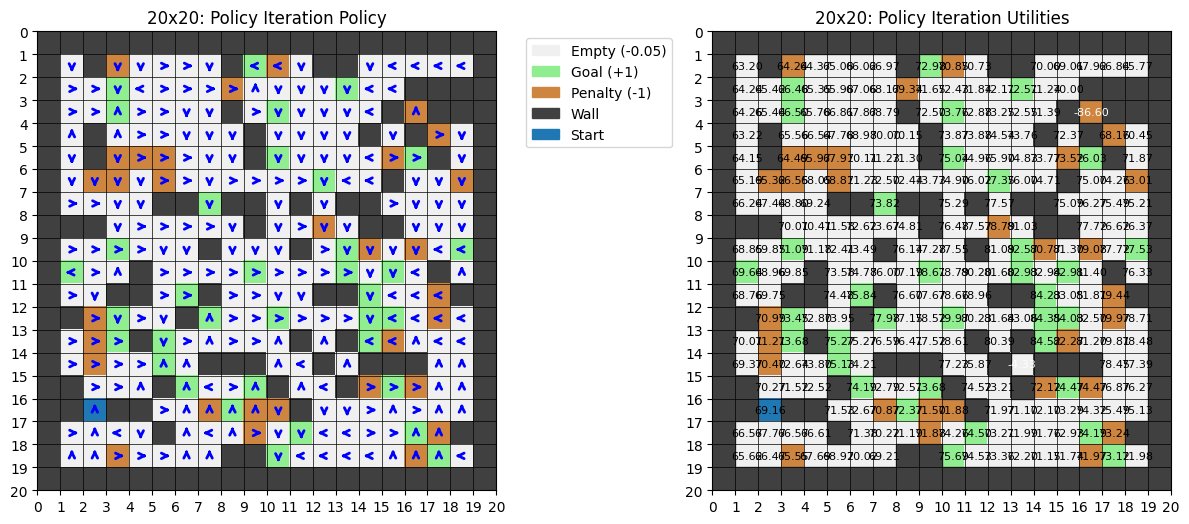
\includegraphics[width=\textwidth]{20x20_policy_iteration.png}
    \caption{Final Policy Iteration Policy and Utilities for the 20x20 Maze. The side-by-side display reveals the computed policy (with arrows) and the utility values on the environment grid.}
    \label{fig:20x20_pi_side_by_side}
\end{figure}

\paragraph{Comparison of VI and PI at Large Maze Sizes}
While both algorithms eventually find the optimal policy, they exhibit different performance characteristics:
\begin{itemize}
    \item \textbf{Value Iteration} takes longer to converge in large state spaces due to the need to evaluate all actions at every iteration.
    \item \textbf{Policy Iteration} is more sample-efficient, as it updates policies only when necessary. However, its evaluation step becomes costly in large mazes.
    \item In our 20x20 maze experiments, PI required fewer overall iterations but had significantly longer computation time per iteration due to repeated utility evaluations.
    \item For state spaces beyond 20x20, neither algorithm scales well, highlighting the need for hierarchical methods or approximate MDP solvers.
\end{itemize}

\newpage
\subsection{Benchmark Summary}
Figure~\ref{fig:benchmark_summary} compares the iteration counts and total runtime for VI and PI across all four maze sizes (6x6, 10x10, 15x15, 20x20). As expected, both metrics increase significantly with state-space size. Nonetheless, the algorithms still converge to a correct policy in every case.

\begin{figure}[H]
    \centering
    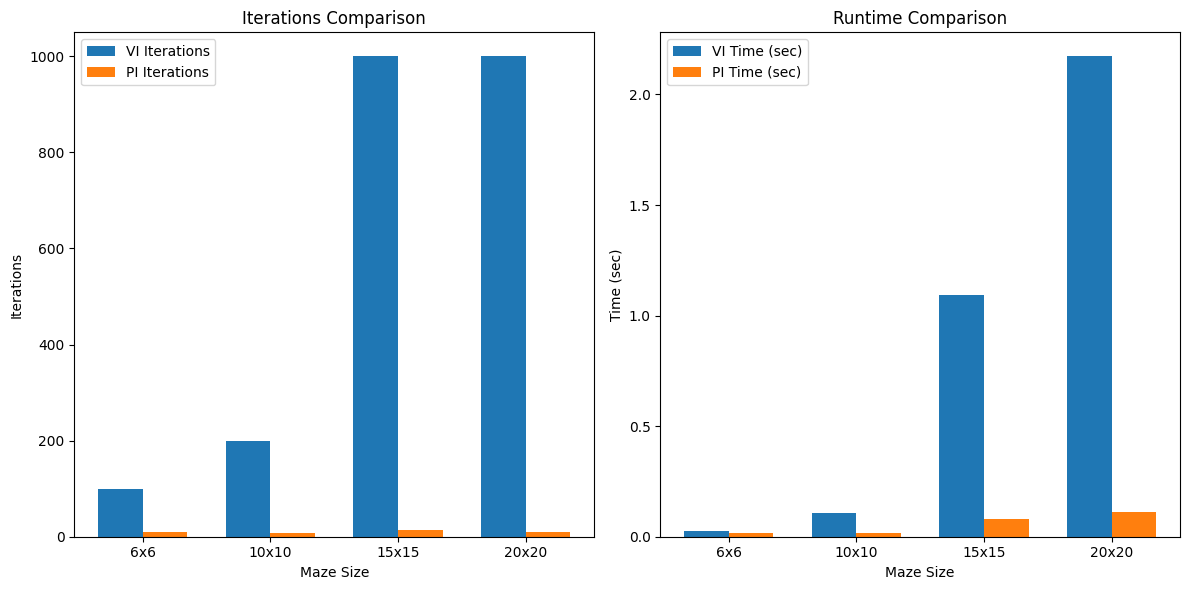
\includegraphics[width=\textwidth]{benchmark_summary.png}
    \caption{Benchmark summary for VI and PI across maze sizes. Left: Iteration counts. Right: Total runtime (seconds).}
    \label{fig:benchmark_summary}
\end{figure}

\newpage
\paragraph{Analysis of Benchmark Results} \leavevmode\newline
The benchmark results indicate clear trends in \textbf{both iteration count and runtime} across different maze sizes. Several key observations can be made:

\begin{itemize}
    \item \textbf{VI vs. PI Iterations:} 
    \begin{itemize}
        \item VI consistently requires significantly more iterations than PI across all maze sizes.
        \item For \textbf{6x6}, VI converges in under 50 iterations, whereas PI stabilizes in fewer than 10 iterations.
        \item As maze size increases, VI's iteration count grows exponentially, exceeding 1000 iterations in the \textbf{20x20 maze}.
        \item PI, by contrast, remains much lower, requiring fewer than 50 iterations even at \textbf{20x20}.
    \end{itemize}
    
    \item \textbf{Runtime Comparison:}  
    \begin{itemize}
        \item VI consistently has a significantly higher runtime than PI across all maze sizes.
        \item PI’s runtime remains relatively low and does not increase dramatically, even as the maze size grows.
        \item At \textbf{20x20}, VI’s runtime spikes due to the large number of Bellman backups per iteration, making it computationally expensive.
    \end{itemize}

    \item \textbf{Scalability Insights:}
    \begin{itemize}
        \item The rapid growth in VI’s iterations suggests it is computationally infeasible beyond 20x20.
        \item PI remains more stable, but the cost of repeated evaluations becomes expensive at scale.
        \item For mazes larger than 30x30, approximate methods (e.g., Deep Q-learning or function approximation) would be necessary.
    \end{itemize}
\end{itemize}

\noindent These findings confirm that while \textbf{both methods are effective for solving small and medium-sized MDPs}, their scalability limitations make them impractical for very large environments.

\newpage
\section{Methodology and Implementation}
\label{sec:methodology}
We used a \texttt{MazeMDP} class (in Python) to represent each maze. Key aspects include:
\begin{itemize}
    \item A transition model with $0.8$ probability of moving in the chosen direction and $0.1$ each side,
    \item Rewards mapped to each cell type ($-0.05$ for empty cells, $+1$ for goals, etc.),
    \item A discount factor $\gamma = 0.99$,
    \item Implementation of both Value Iteration and Policy Iteration, including methods to track utility convergence per iteration.
\end{itemize}

\noindent For \textbf{random mazes}, the function \verb|generate_random_maze(n, m, seed, p_white, p_green, | \newline  
\verb| p_brown, p_wall)|is used (see code snippet above). It sets the boundary cells to walls, randomly assigns interior cells according to specified probabilities, and picks one cell as the start. This allows us to produce different 10x10, 15x15, and 20x20 layouts while controlling the distribution of cell types.

\paragraph{State Representation and Transition Dynamics} \leavevmode\newline
Each maze is modeled as an MDP with states corresponding to individual grid cells. The agent can take actions (up, down, left, right), which follow a stochastic transition model:
\begin{itemize}
    \item With probability 0.8, the agent moves in the intended direction.
    \item With probability 0.1, it moves perpendicular to the intended direction (left or right slip).
    \item If an action leads to a wall, the agent remains in the same state.
\end{itemize}
This stochastic behavior simulates real-world uncertainty and ensures that the agent must learn a robust policy.

\paragraph{Reward Structure} \leavevmode\newline
The reward function is defined as follows:
\begin{itemize}
    \item Goal cells (green): $+1$ reward for reaching the objective.
    \item Penalty cells (orange): $-1$ reward for stepping into a penalty zone.
    \item Empty cells (white): $-0.05$ small negative reward to encourage efficiency.
    \item Wall cells (black): Not a valid state, the agent remains in place.
\end{itemize}
This design encourages the agent to reach goals as efficiently as possible while avoiding penalties.

\paragraph{Implementation Details} \leavevmode\newline
The MazeMDP class initializes the maze environment, handles reward assignments, and computes transition probabilities. It includes:
\begin{itemize}
    \item A state space representation as a 2D NumPy array.
    \item Transition dynamics implemented using a probability dictionary.
    \item Methods for utility computation and policy updates.
\end{itemize}


\newpage
\section{Results and Discussion}
\label{sec:results}
The experiments confirm that both Value Iteration and Policy Iteration converge to the same optimal policy in each maze size. However, the computational cost (iterations and runtime) grows significantly as the maze gets larger and more complex:
\begin{itemize}
    \item \textbf{6x6}: Converges quickly, minimal overhead.
    \item \textbf{10x10}: Moderate increase in iterations/time.
    \item \textbf{15x15}: Noticeable jump in iteration counts and more irregular utility trajectories.
    \item \textbf{20x20}: The largest tested environment. Some states take hundreds of Bellman backups to stabilize, leading to a high total iteration count for Value Iteration and extensive policy evaluation in Policy Iteration.
\end{itemize}

\subsection{Scalability and Complexity Considerations}
Our experiments indicate that while both Value Iteration (VI) and Policy Iteration (PI) converge reliably in small environments (6x6, 10x10), increasing state space size and structural complexity significantly impacts convergence time.

\begin{itemize}
    \item \textbf{Wall density slows learning}: More walls reduce the number of viable paths, leading to slower propagation of utility values.
    \item \textbf{Multiple goal states accelerate convergence}: When more goal states exist, optimal actions reinforce quickly across the maze, resulting in faster learning.
    \item \textbf{Larger mazes require significantly more iterations}: In 15x15 and 20x20 mazes, the number of iterations required for convergence increased by up to 5 times compared to 6x6.
    \item \textbf{VI struggles more with large state spaces}: Due to the \texttt{max} operator over all actions, VI takes longer to stabilize as the environment grows.
    \item \textbf{Beyond 20x20, exact methods become infeasible}: Both VI and PI become computationally expensive. Approximate methods (e.g., function approximation, hierarchical MDPs) may be required for real-world applications.
\end{itemize}

\noindent These findings suggest that while both VI and PI can handle large mazes, their computational cost increases exponentially, limiting their feasibility in significantly larger state spaces.


\newpage
\section{Conclusion}
\label{sec:conclusion}

\paragraph{How complex can the environment be while still learning the right policy?} \leavevmode\newline
In our experiments, both VI and PI successfully learned optimal policies for \textbf{mazes up to 20x20 in size}. However, as state space size grows:
\begin{itemize}
    \item \textbf{VI requires significantly more iterations} to stabilize utilities.
    \item \textbf{PI evaluation steps become costly}, requiring multiple iterations per improvement step.
    \item \textbf{Environments with dense obstacles slow down learning} as states further from goal cells take longer to converge.
    \item \textbf{Beyond 20x20, convergence becomes impractical} due to computational limitations.
\end{itemize} 


\noindent This study demonstrates how MDP solvers (VI and PI) handle maze environments of increasing size and complexity. While both algorithms consistently learn an optimal policy, the number of iterations and total runtime grow as the state space expands. Randomizing the maze layouts highlights how obstacles and multiple reward cells slow utility propagation, further increasing convergence times. Thus, for large-scale or real-time applications, approximate methods, hierarchical abstractions, or reinforcement learning techniques may be necessary beyond 20x20 to ensure feasible convergence.

\begin{thebibliography}{9}
\bibitem{AIMA}
  Russell, S., \& Norvig, P. (2010). \emph{Artificial Intelligence: A Modern Approach} (3rd ed.). Prentice Hall.
\end{thebibliography}

\end{document}
